\section{Results}




\subsection{Probability distribution}

The probability distribution of energy (\cref{fig:distribution}) shows that
at low temperature almost all of the states are in a low energy state.
As the temperature and the variance increases the distribution becomes more
spread out.

\begin{figure}[H]
  \centering
  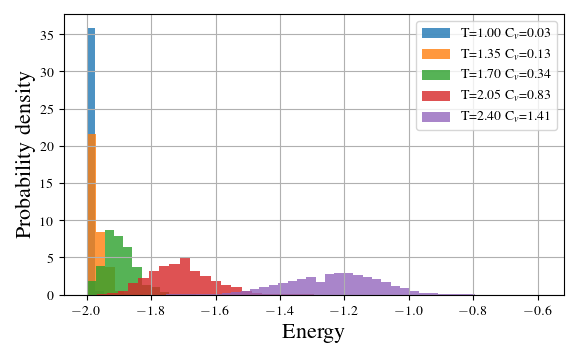
\includegraphics[width=\textwidth]{../figures/distribution.png}
  \caption{Probability distribution of energy, scaled with number of spins. L=20}
  \label{fig:distribution}
\end{figure}




\subsection{Phase transitions}




\begin{figure}[H]
  \centering
  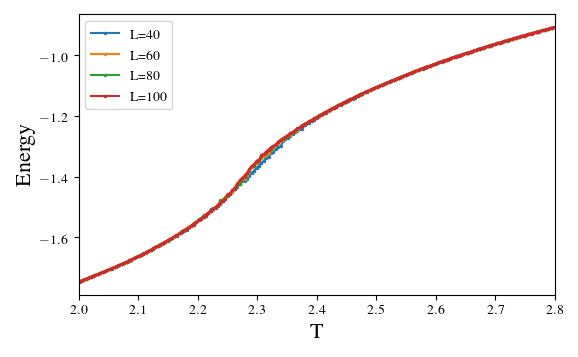
\includegraphics[width=\textwidth]{../figures/phase_E.png}
  \caption{$\Delta$ T=0.05}
  \label{fig:phase_E}
\end{figure}

\begin{figure}[H]
  \centering
  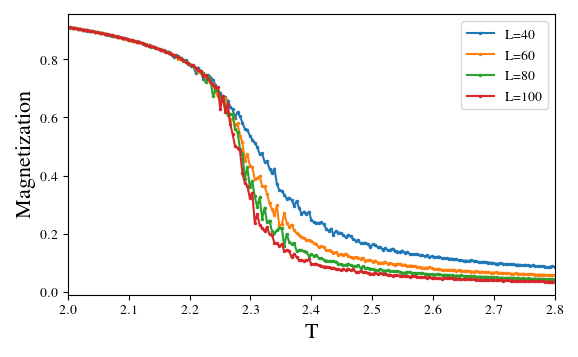
\includegraphics[width=\textwidth]{../figures/phase_Mabs.png}
  \caption{}
  \label{fig:phase_Mabs}
\end{figure}



\begin{figure}[H]
  \centering
  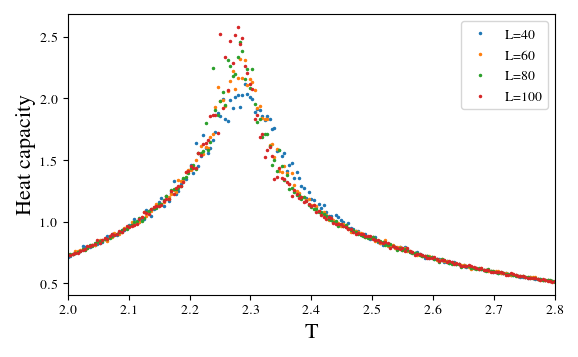
\includegraphics[width=\textwidth]{../figures/phase_cv.png}
  \caption{}
  \label{fig:phase_cv}
\end{figure}


\begin{figure}[H]
  \centering
  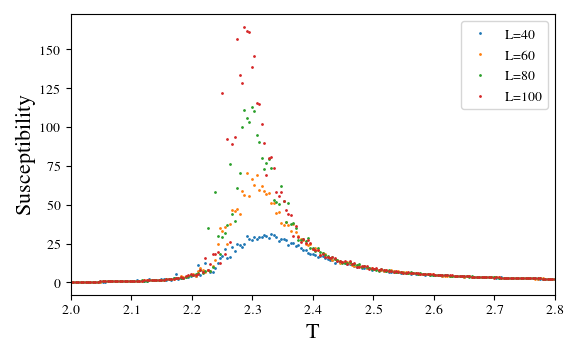
\includegraphics[width=\textwidth]{../figures/phase_suscept.png}
  \caption{}
  \label{fig:phase_suscept}
\end{figure}
